\documentclass{article}
\usepackage[utf8]{inputenc}
%\usepackage{subcaption} %Captions for subfigure?
\paperheight=297mm % A4 paper dimensions
\paperwidth=210mm
\usepackage{float}

% Manually setting page dimensions
\setlength{\textheight}{235mm}
\setlength{\topmargin}{-1.2cm} 
\setlength{\textwidth}{15.5cm}
\setlength{\oddsidemargin}{0.5cm}
\setlength{\evensidemargin}{0.5cm}

% Include more figures type: eps,pdf,jpg, png
\usepackage{graphicx}
\usepackage[table,xcdraw]{xcolor}

% Hyperlinks:
\usepackage[hidelinks,colorlinks=false,bookmarks=false,linkcolor=black,urlcolor=black]{hyperref}

\pdfminorversion=5 
\pdfcompresslevel=9
\pdfobjcompresslevel=2\pdfobjcompresslevel=2


\begin{document}
\begin{center}
\textbf{\LARGE{Elevation encoder cable}}\\
Alexander Pollak  and Marc Jacquart\\
March 13th, 2024\\
\end{center}


This document describes the wiring of the elevation encoder cable D-Sub 9-pin (DB9) connector. Figure \ref{fig:picture_parts} shows a picture of the tool and parts needed. Figure \ref{fig:diagram_connector} shows a wiring diagram for the D-Sub 9-pin connector.

List of parts and tool needed:
\begin{itemize}
\item D-Sub contact pins (TE\#: 66682-2)
\item D-Sub 9-pin connector (TE\#: 205204-9, Newark\#: 16M2875)
\item Crimp tool (TE\#: 354940-1)
\end{itemize}

\begin{figure}[H]
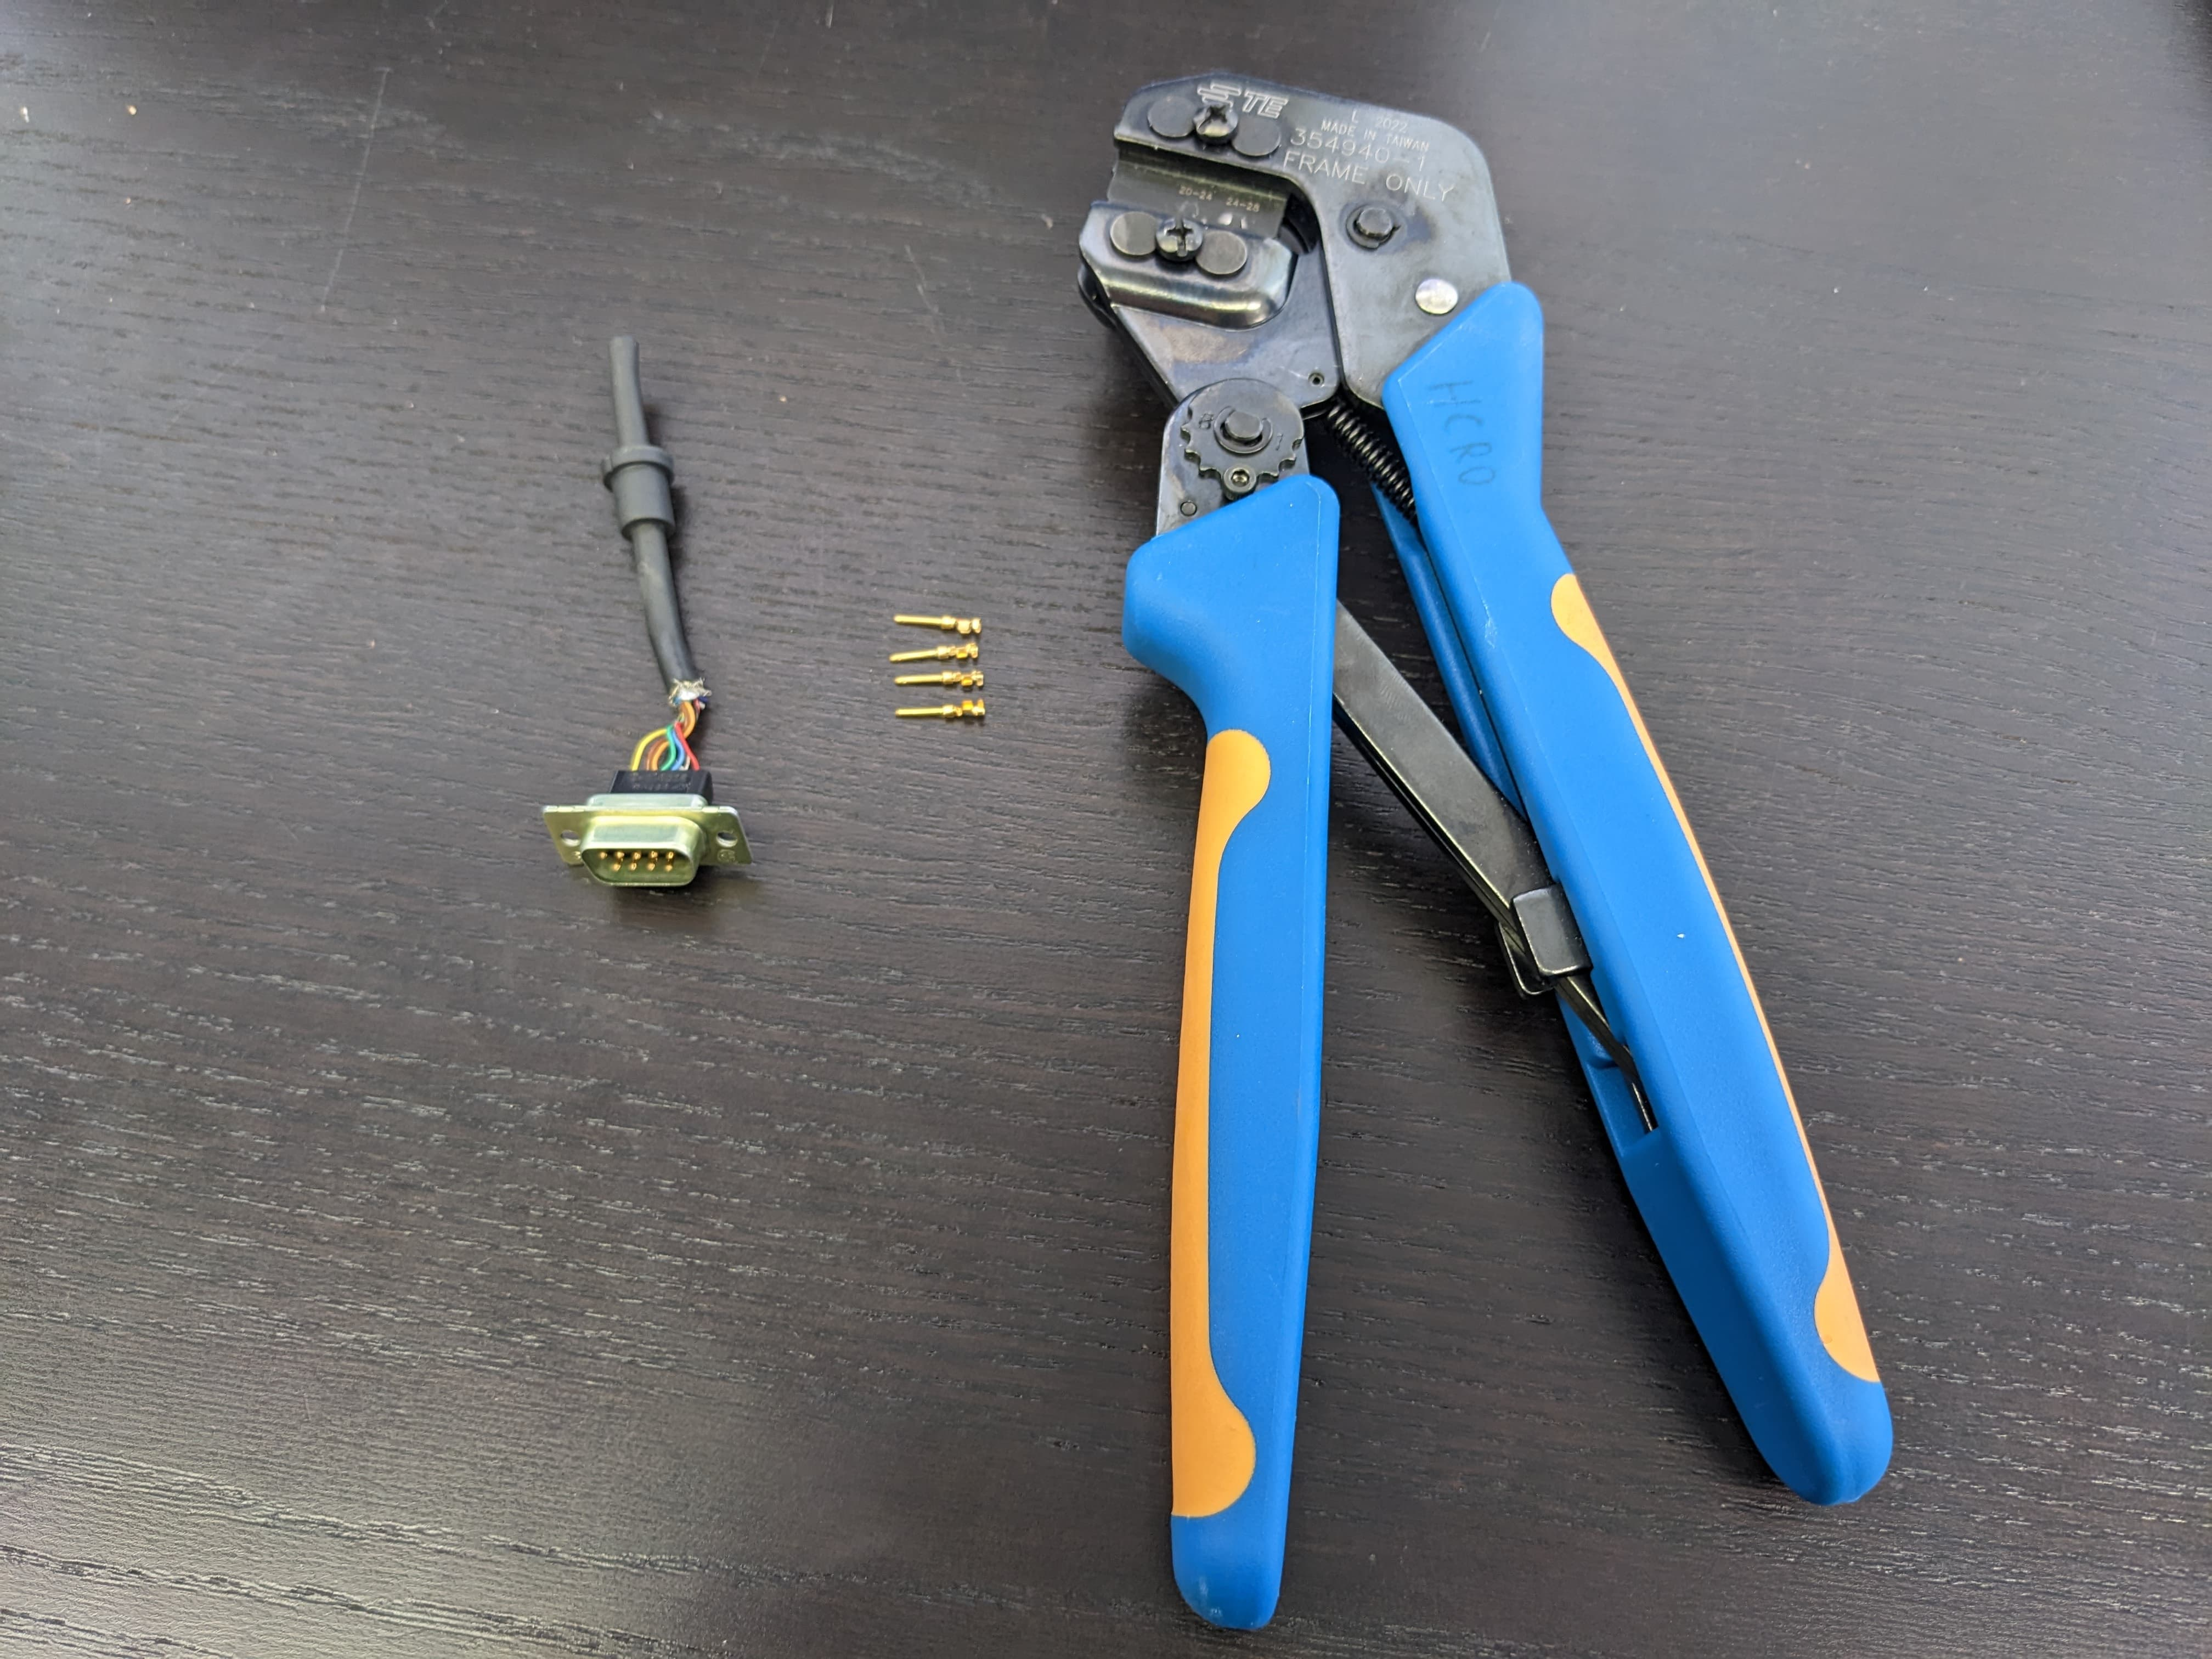
\includegraphics[width=\textwidth]{images/connector_crimp_tool.jpeg}
\caption{Picture of the tool and parts needed to make an elevation encoder cable connector.}
\label{fig:picture_parts}
\end{figure}

\begin{figure}[H]
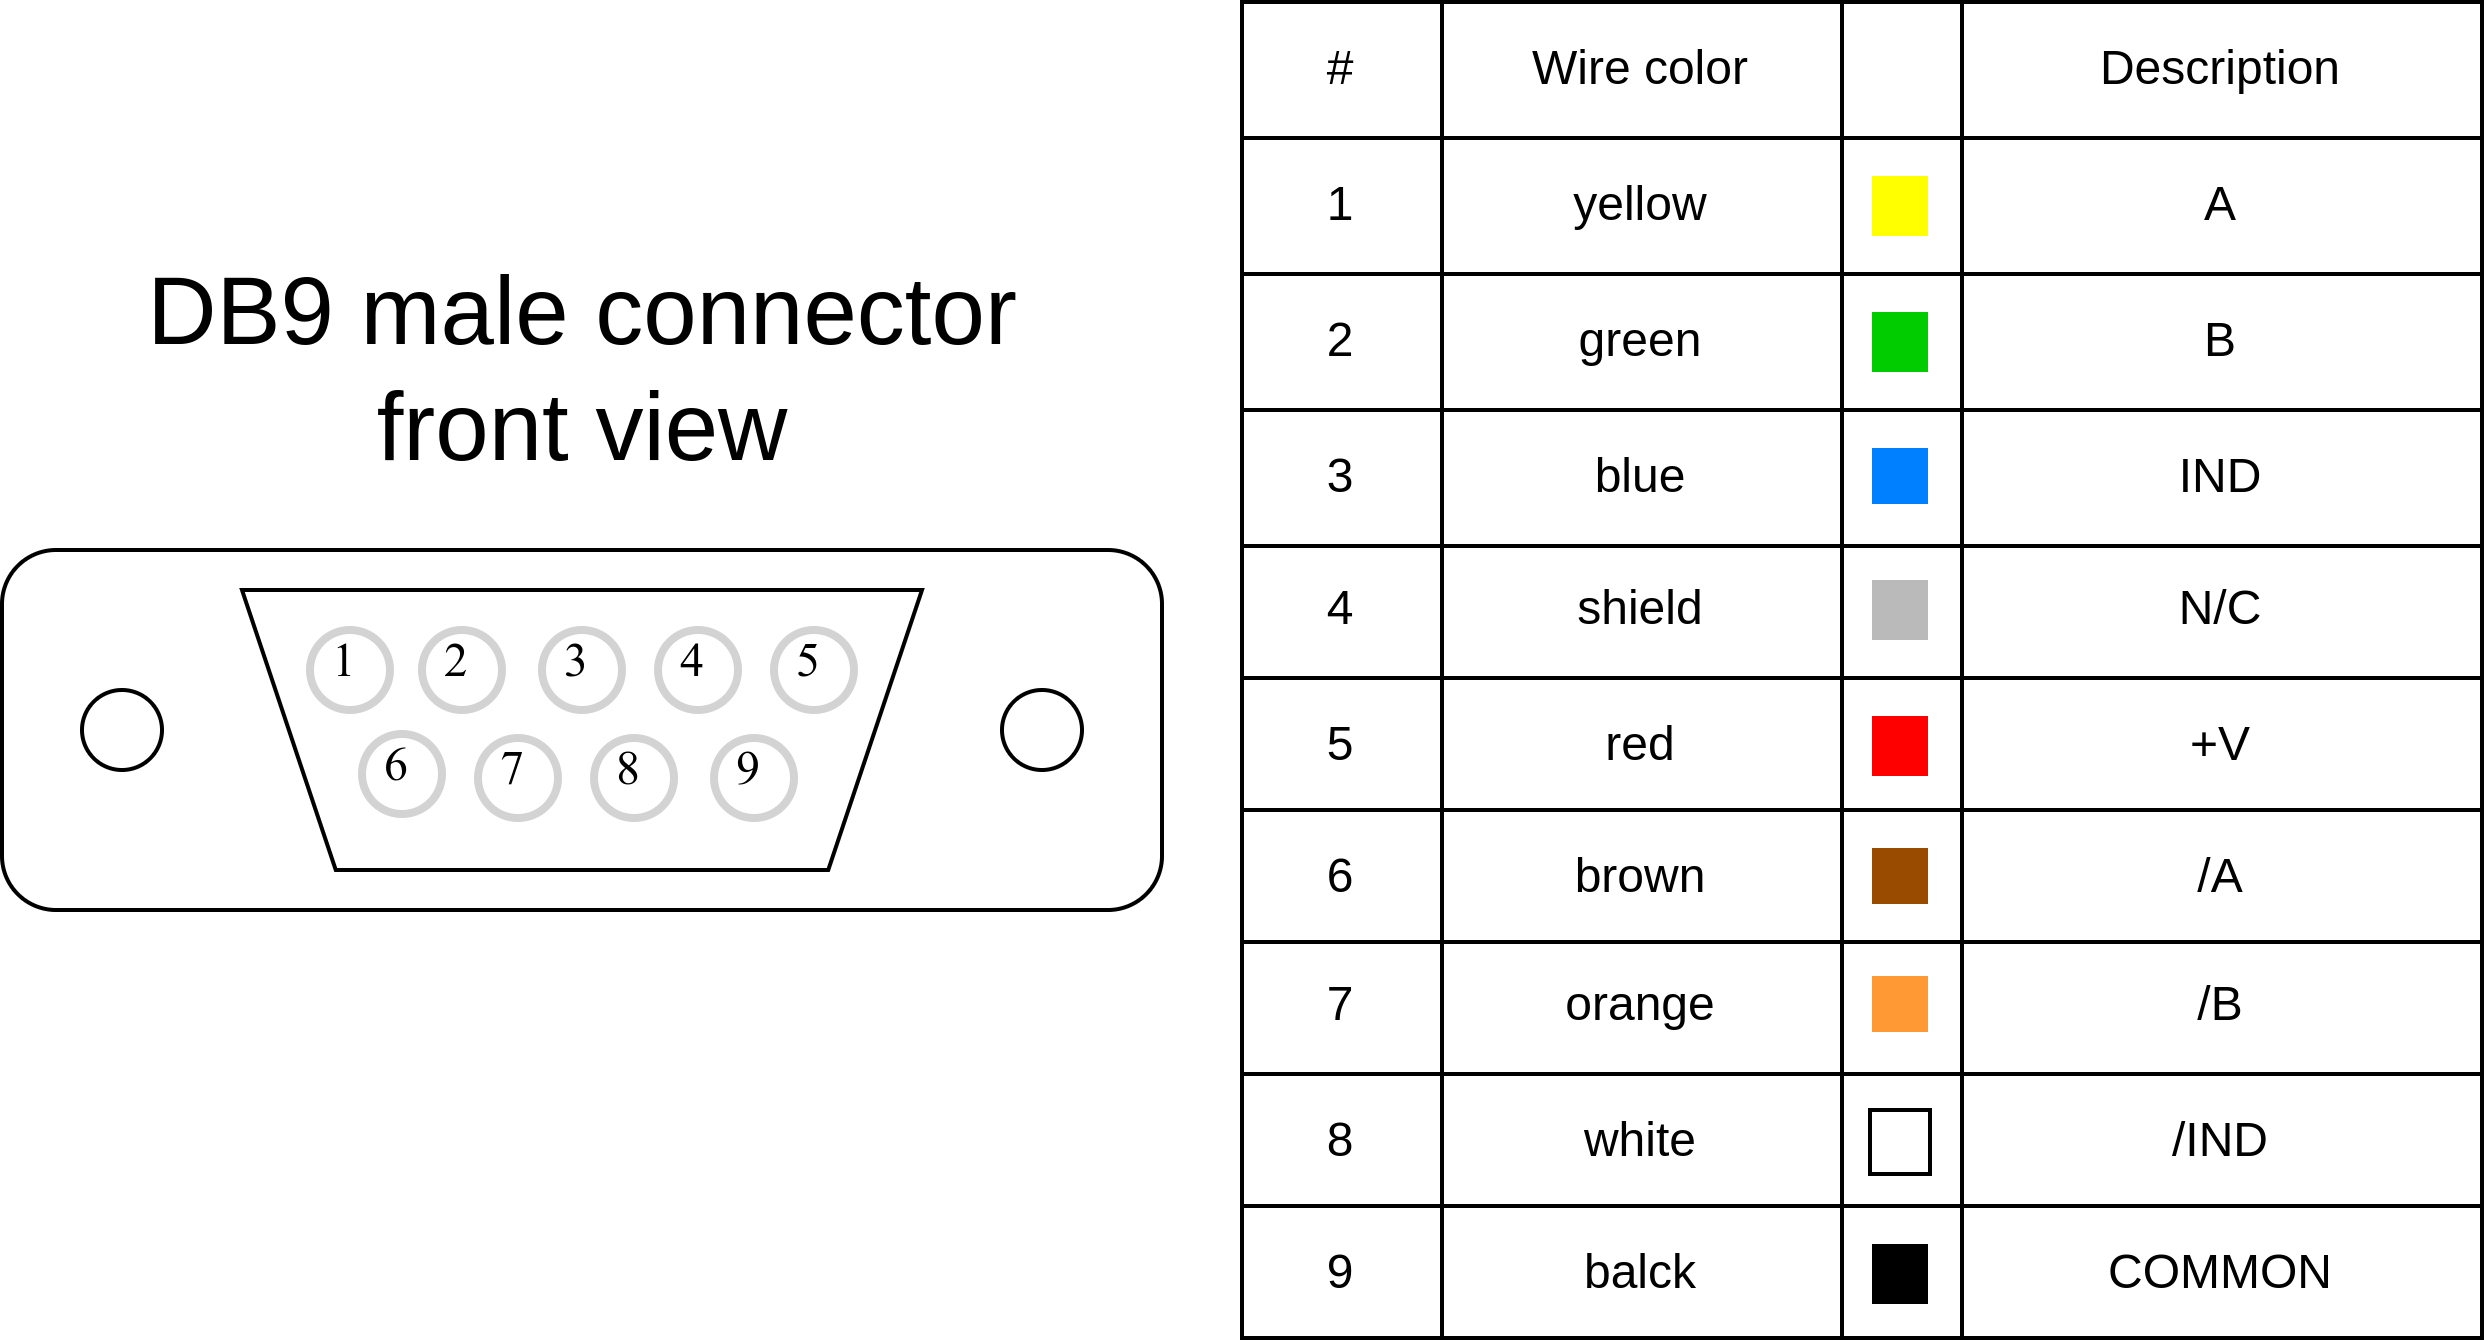
\includegraphics[width=\textwidth]{images/schematics/DB9_connector.png}
\caption{D-Sub 9-pin connector wiring diagram.}
\label{fig:diagram_connector}
\end{figure}
\end{document}